\section{Visual Design}
\label{sec:interface}

\subsection{Event}
An event is represented by a rounded rectangle with a short text inside summarizing its content. All rectangles have the same height to provide a consistent appearance, especially when they are later connected to form a schema (Section \ref{sub:schema-outline}). Rectangles are assigned the same maximum width and long texts are trimmed to fit into their rectangles. The full content of an event will be displayed when it is hovered. Events can include categorical attributes. For example, in news reports, the themes of an article can be sport, fashion or both. Inside the border of an event, small colored rectangles are added to the left of its text to indicate its categories. Note that only around 12 colors can be distinguished simultaneously in the human view~\cite{Munzner2014}. We choose Set 1 of qualitative colors from ColorBrewer~\cite{Harrower2003} for the colormap. The eight most appeared categories are displayed using these colors and other categories share the same different color. Figure~\ref{fig:event} shows an example of event with three color-coded categories.

\begin{figure}[!htb]
\centering
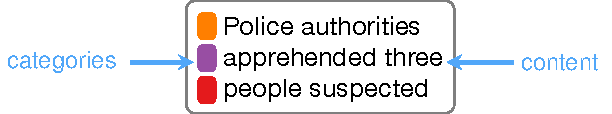
\includegraphics[width=.35\columnwidth]{event}
\caption{An event with three categories. The event is represented as a rounded rectangle with summarized content inside. On the left side of the text, small color-coded rectangles indicate its categories. The event is positioned along the time axis at which it happens -- 8th of May.}
\label{fig:event}
\end{figure}

An event is left-aligned with its temporal value on the time axis. To reduce cluttering, an event is not visually connected to its corresponding point on the axis. Instead, when the mouse hovers an event, its time point is highlighted. The time axis is shown as a horizontal line at the bottom of all events. It includes two hierarchical temporal scales, which are changed dynamically according to the range of the displayed events. For example, Figure~\ref{fig:event} shows two scales: ``month/day'', but they can switch to ``year/month'' if the range is larger.

\subsection{Schema}
r of relevant events or pieces of evidence, the analyst starts combining them to form a \textit{schema}. A schema is a set of related events that are connected to each other in a certain way. For example, a schema might contain all events about a particular person. Figure~\ref{fig:schema} shows examples of schema. 

\begin{figure}[ht]
	\centering
	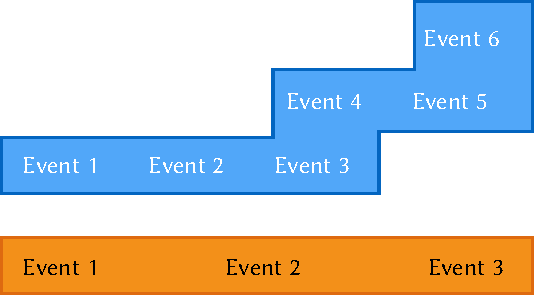
\includegraphics{schema}
	\caption{.}
	\label{fig:schema}
\end{figure}

\begin{figure}[ht]
\centering
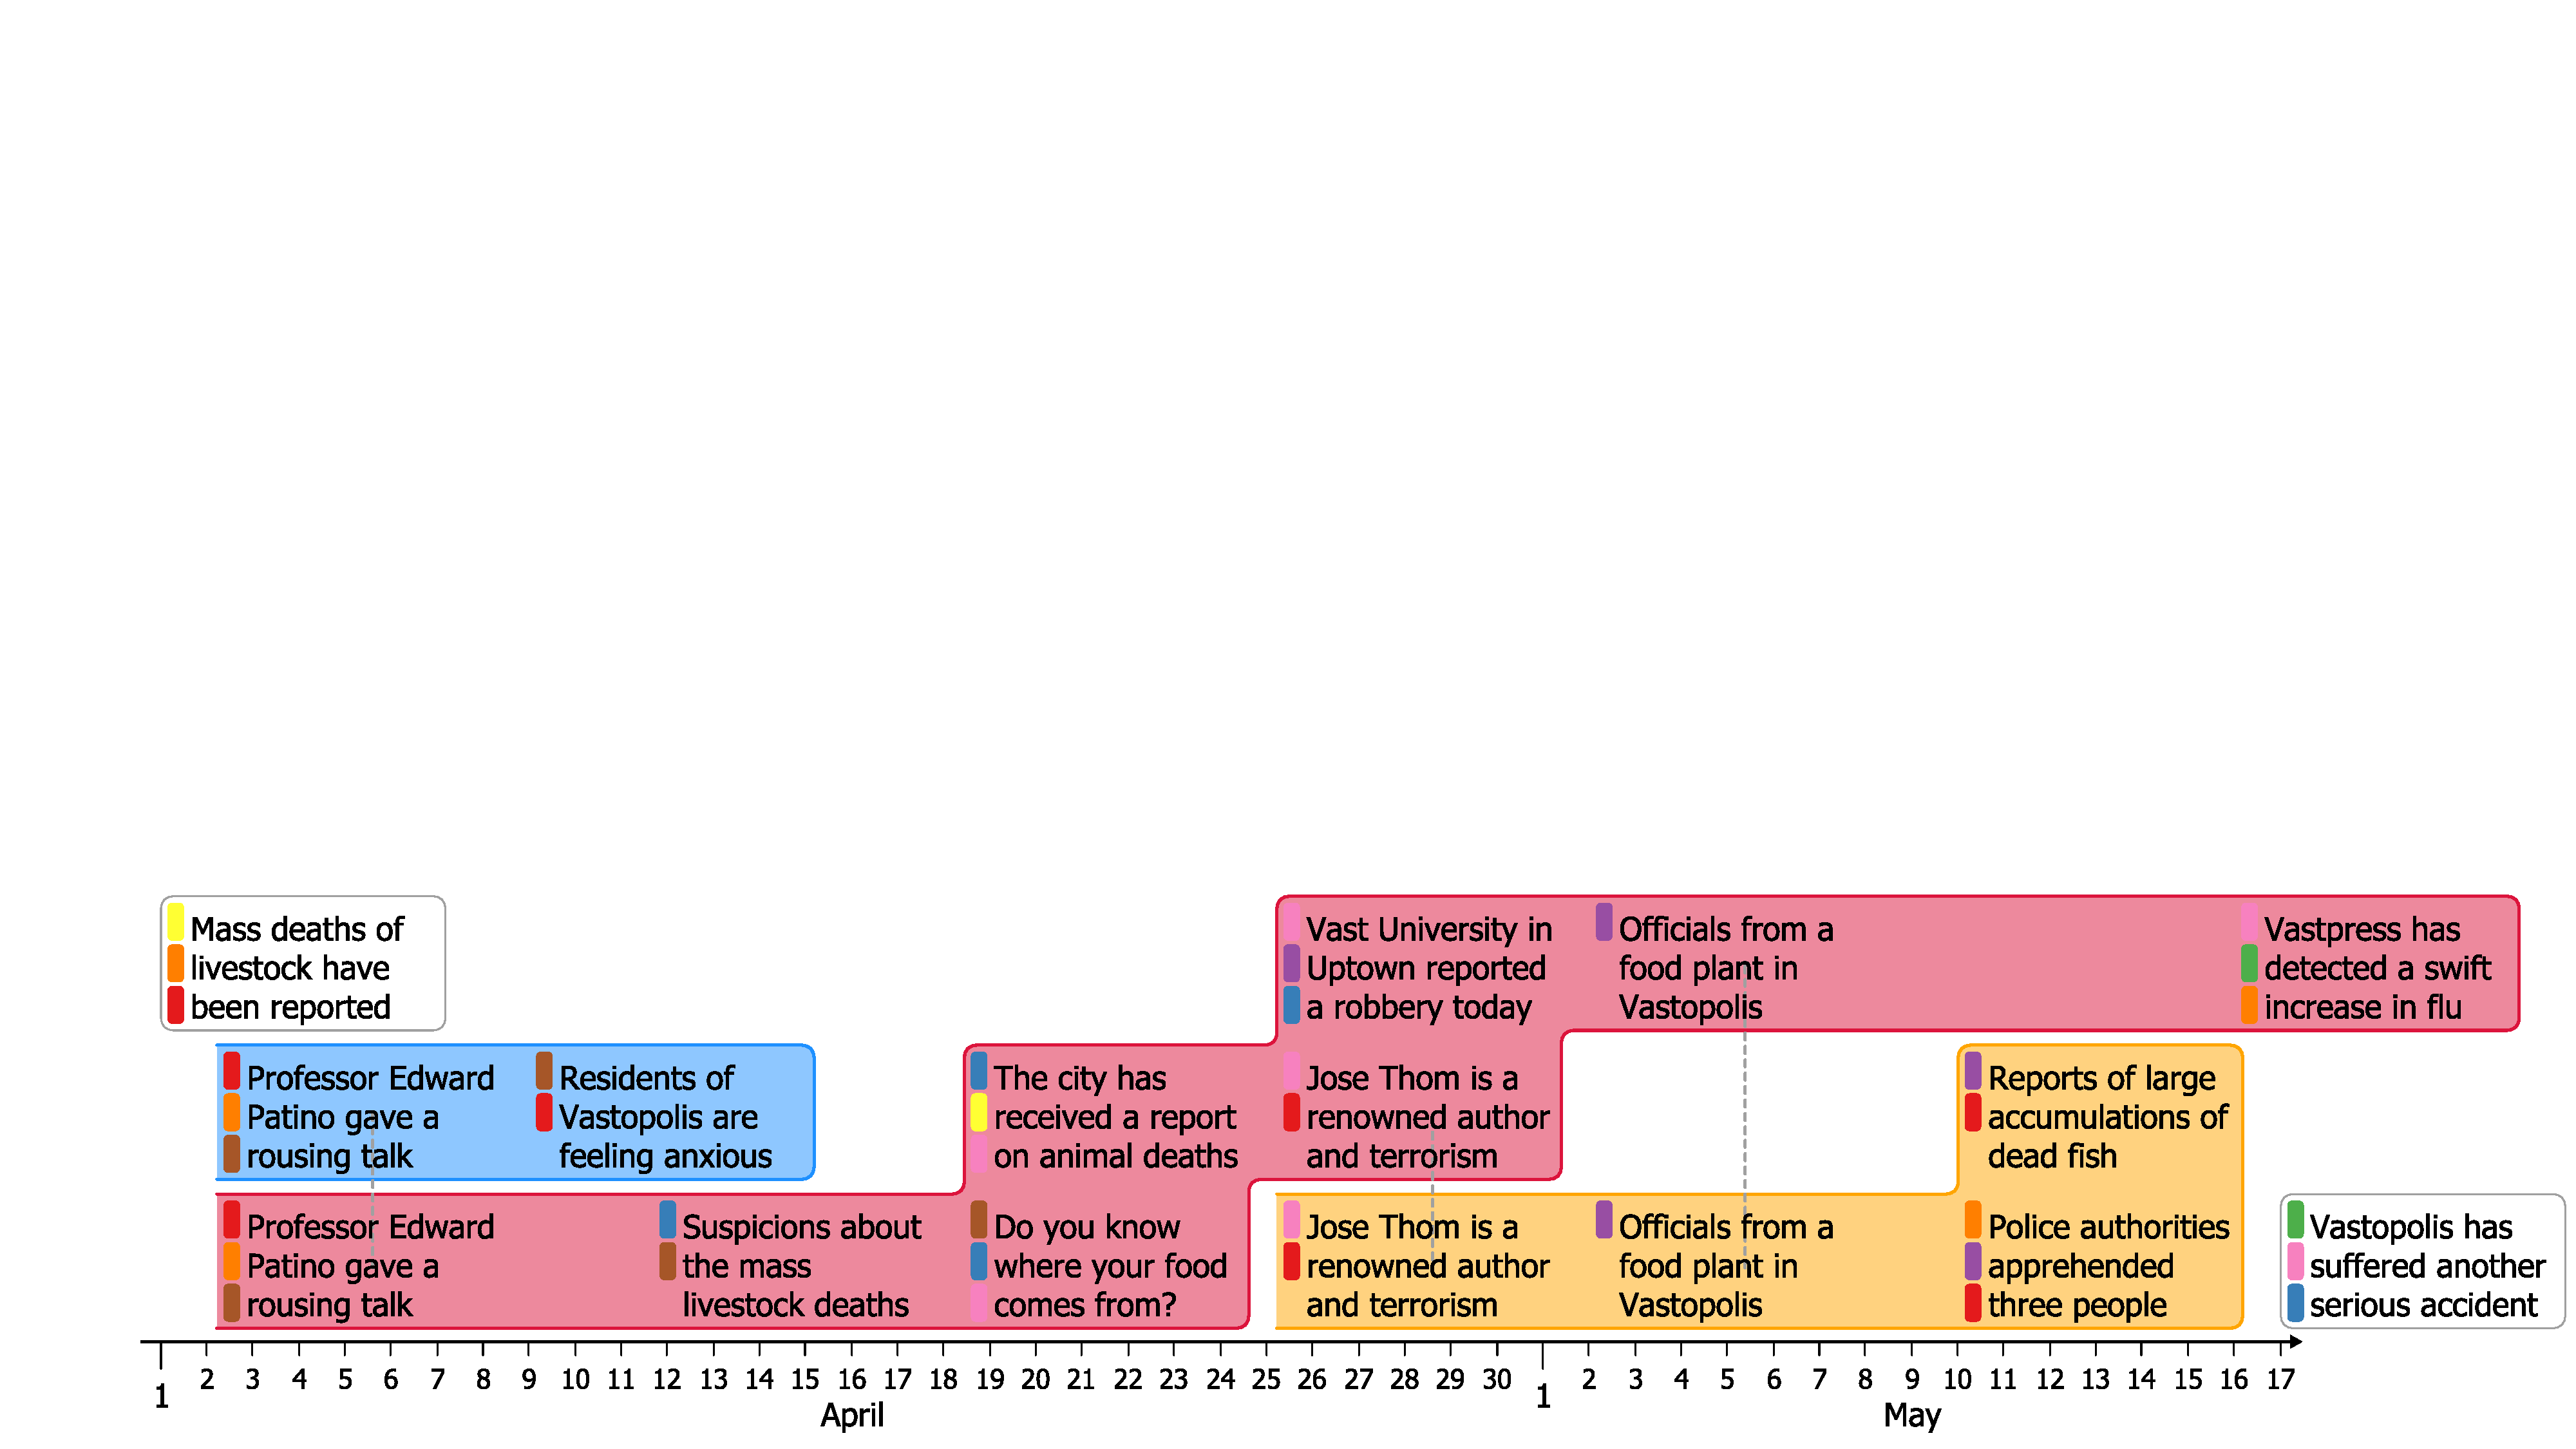
\includegraphics[width=\linewidth]{teaser}
\caption{SchemaLine: each piece of text is an analyst note, positioned along the time axis at which the event happened. Related notes are linked together to form a ``schema'' or ``frame''. There are three frames in this example represented as colored rectilinear paths. Small color-coded rectangles on the left side of notes are ``categories''.}
\label{fig:teaser}
\end{figure}

We consider several design options to connect events within a schema such as using colored/shaped icons or node-link diagrams. However, they all have some drawbacks as discussed in the Related work (Section~\ref{sec:relatedwork}). Computational methods that allow visualize a large number of events with different themes such as ThemeRiver~\cite{Havre2002} do not work either because individual events and interactions are more essential in SchemaLine. \note{I don't quite understand what the `computational' means and the argument follows} Also, it should be easy to follow events within a schema in temporal order. We decided to visualize each schema as a colored stripe, which is inspired by Munroe's hand-drawn visualization~\cite{Munroe2009}. A character line in Munroe's work connects all events happened to that character. Similarly, our schema is a color stripe connecting all events belonging to it. Instead of using a thin line, we use a path with unique width (an event's height) to make enough space to display the event's summary text and allow interaction with individual notes. A rectilinear path is employed to provide a nice visualization rather than direct connection between events. 